\section{Introduction}

% for placement
\begin{figure*}[ht]
    \centering
    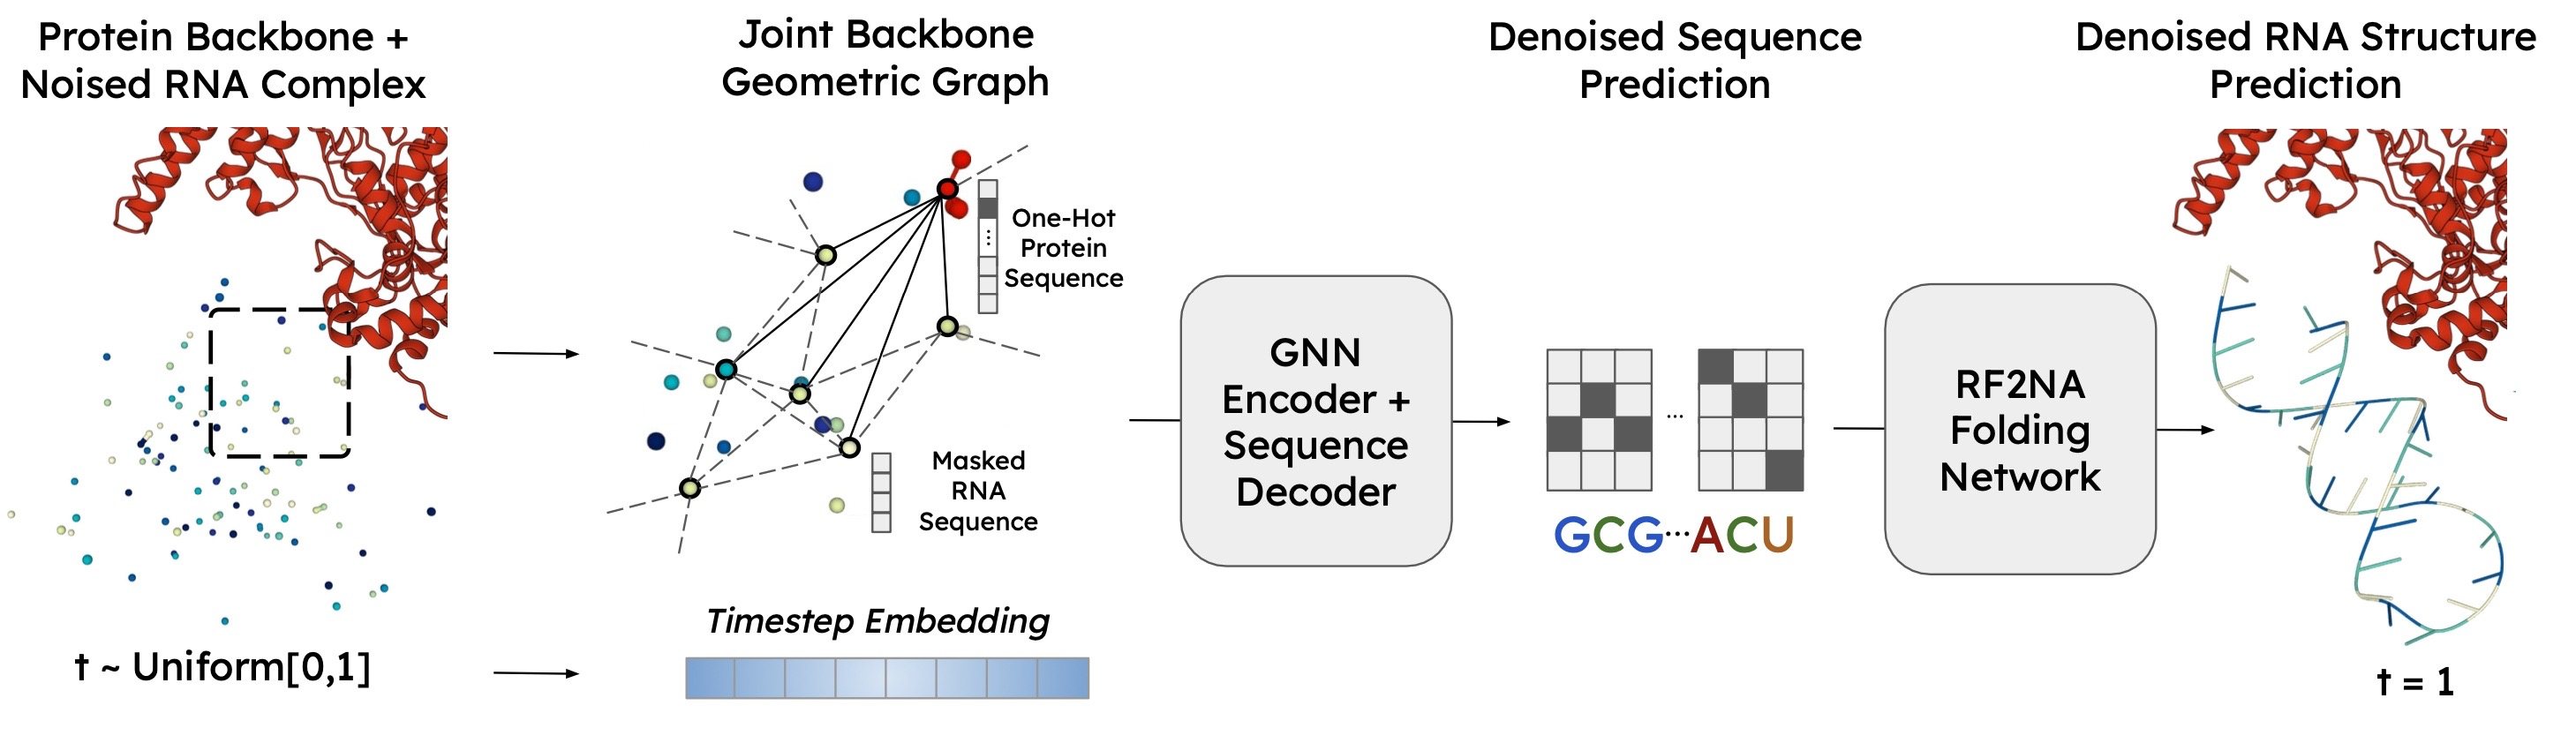
\includegraphics[width=2\columnwidth]{if-flow-match.png}
    \caption{One forward pass in RNAFlow training, during which an inverse folding model is finetuned to be the flow matching score prediction network. The inverse folding model predicts a denoised RNA sequence from a noised complex backbone graph. The predicted sequence is folded by RF2NA for sequence and structure supervision.}
    \label{fig:1}
\end{figure*}

In recent years, RNA molecules have been engineered for versatile and controllable functions in biological systems \cite{dykstra2022engineering}, ranging from synthetic riboswitch sensors that modulate gene expression to aptamers that bind with protein targets ~\cite{thavarajah2021rna, vezeau2023automated, keefe2010aptamers}. However, experimental methods for high-throughput RNA selection like SELEX~\cite{gold2015selex} remain time-consuming and labor-intensive. To unlock the full potential of RNA therapeutics, there is a pressing need for developing deep learning models to automatically design RNAs that bind with a protein of interest \cite{sanchez2019rna}.

Current state-of-the-art biomolecular structure design methods are based on diffusion models~\cite{ho2020denoising,yim2023se} or flow matching~\cite{lipman2022flow,bose2023se}. For example, RFDiffusion~\cite{watson2023novo} fine-tuned RoseTTAFold~\cite{baek2021accurate} to generate novel protein structures that meet complex constraints, including conditional generation of protein binders. While we can adopt a similar approach for conditional RNA structure generation by fine-tuning a protein-nucleic acid structure prediction network like RoseTTAFold2NA (RF2NA)~\cite{baek2023accurate}, there are two major caveats. First, RNAs exhibit a high degree of conformational flexibility, which is often the key to their biological function \cite{ganser2019roles}. A generative model that outputs a single static structure may bottleneck the downstream sequence generation process, since an ideal sequence should account for desired RNA dynamics. Second, fine-tuning a large structure prediction network is computationally expensive, motivating a method that applies a pre-trained model like RF2NA directly. 

In this paper, we propose RNAFlow, a flow matching model for RNA sequence-structure design. The denoising network in RNAFlow is composed of an RNA inverse folding model and a pre-trained RF2NA network. In each iteration, RNAFlow first generates a RNA sequence given a noisy protein-RNA complex and then uses RF2NA to fold into a denoised RNA structure. For computational efficiency, we train the inverse folding model to minimize the flow matching objective while keeping RF2NA fixed. RNAFlow offers three advantages over previous methods like RFDiffusion. First, RNAFlow generates an RNA sequence and its structure simultaneously. Second, it is much easier to train because we do not fine-tune a large structure prediction network. Third, our framework enables us to model the dynamic nature of RNA structures for inverse folding. Specifically, we utilize the final few structure predictions from inference trajectories as an effective approximation of an RNA conformational ensemble and enhance our inverse folding model to condition on dynamic RNA conformations.

We evaluate our method on the task of protein-conditioned RNA structure and sequence generation. RNAFlow outperforms a standard sequence-only approach and a recent diffusion model \cite{morehead2023towards} for nucleic acid sequence-structure generation in terms of native sequence recovery, RMSD, and lDDT. Additionally, we show that RNAFlow can be used in the motif-scaffolding setting to generate plausible RNA aptamers for G-protein-coupled receptor kinase 2 (GRK2), a target with known sequence motif for GRK2 binding.